\section{常微分方程}

	\begin{ti}
		微分方程 $3 \ee^{x} \tan y \dd{x} + \bigl( 1 - \ee^{x} \bigr) \sec^{2}y \dd{y} = 0$ 的通解是\htwo.
	\end{ti}

	\begin{ti}
		微分方程 $y' \tan x = y \ln y$ 的通解是\htwo.
	\end{ti}

	\begin{ti}
		已知曲线 $y = y(x)$ 经过点 $\bigl( 1,\ee^{-1} \bigr)$,且在点 $(x,y)$ 处的切线在 $y$ 轴上的截距为 $xy$,求该曲线方程的表达式.
	\end{ti}

	\begin{ti}
		求方程 $\frac{\dd{y}}{\dd{x}} = \bigl( 1 - y^{2} \bigr) \tan x$ 的通解以及满足 $y(0) = 2$ 的特解.
	\end{ti}

	\begin{ti}
		微分方程 $x \dd{y} = \bigl( y - \sqrt{x^{2} + y^{2}} \bigr) \dd{x}(x > 0)$ 满足 $y(1) = 0$ 的特解是\kuo.

		\twoch{$\sqrt{x^{2} + y^{2}} + y = x$}{$\sqrt{x^{2} + y^{2}} + y = 1$}{$\sqrt{x^{2} + y^{2}} - y = x$}{$\sqrt{x^{2} + y^{2}} - y = 1$}
	\end{ti}

	\begin{ti}
		求微分方程 $\bigl( 1 + \ee^{-\frac{x}{y}} \bigr) y \dd{x} + (y - x) \dd{y} = 0$ 的通解.
	\end{ti}

	\begin{ti}
		求微分方程 $xy' + y = x\ee^{x}$ 满足 $y(1) = 1$ 的特解.
	\end{ti}

	\begin{ti}
		求 $(4 - x + y) \dd{x} - (2 - x - y) \dd{y} = 0$ 的通解.
	\end{ti}

	\begin{ti}
		求微分方程 $\Bigl( x \frac{\dd{y}}{\dd{x}} - y \Bigr) \arctan \frac{y}{x} = x$ 的通解.
	\end{ti}

	\begin{ti}
		求微分方程 $\bigl( y + \sqrt{x^{2} + y^{2}} \bigr) \dd{x} = x \dd{y}$ 的通解,并求满足 $y(1) = 0$ 的特解.
	\end{ti}

	\begin{ti}
		微分方程 $\bigl( y^{2} + 1 \bigr) \dd{x} = y (y - 2x) \dd{y}$ 的通解是
		
		\noindent\htwo.
	\end{ti}

	\begin{ti}
		已知 $\int_{0}^{1} f(tx) \dd{t} = \frac{1}{2} f(x) + 1$,则 $f(x) = $\htwo.
	\end{ti}

	\begin{ti}
		设 $a > 0$,函数 $f(x)$ 在 $[0,+\infty)$ 内连续有界,证明:微分方程 $y' + ay = f(x)$ 的解在 $[0,+\infty)$ 内有界.
	\end{ti}

	\begin{ti}
		设 $\varphi(x)$ 是以 $2\uppi$ 为周期的连续函数,且 $\varPhi'(x) = \varphi(x), \varPhi(0) = 0$.
		\begin{enumerate}
			\item 求方程 $y' + y \sin x = \varphi(x) \ee^{\cos x}$ 的通解;\label{8.14:1}
			\item 在(\ref{8.14:1})中方程是否有以 $2\uppi$ 为周期的解?若有,请写出所需条件,若没有,请说明理由.
		\end{enumerate}
	\end{ti}

	\begin{ti}
		设方程 $y' + P(x)y = x^{2}$,其中 $P(x) = \begin{cases}
			1, & x \leq 1,\\
			\frac{1}{x}, & x > 1.
		\end{cases}$ 试求在 $(-\infty,+\infty)$ 内的连续函数 $y = y(x)$,使之在 $(-\infty,1)$ 和 $(1,+\infty)$ 内都满足方程,且满足初值条件 $y(0) = 2$.
	\end{ti}

	\begin{ti}
		微分方程 $\frac{\dd{y}}{\dd{x}} = \frac{2xy}{x^{2} + y}$ 的通解为\htwo.
	\end{ti}

	\begin{ti}
		求微分方程 $y' \cos y = (1 + \cos x \sin y)\sin y$ 的通解.
	\end{ti}

	\begin{ti}
		微分方程 $y'' - 6y' + 8y = \ee^{x} + \ee^{2x}$ 的一个特解应具有形式(其中 $a,b$ 为常数)\kuo.

		\twoch{$a \ee^{x} + b \ee^{2x}$}{$a \ee^{x} + b x \ee^{2x}$}{$a x \ee^{x} + b \ee^{2x}$}{$a x \ee^{x} + b x \ee^{2x}$}
	\end{ti}

	\begin{ti}
		微分方程 $y'' - 4y' + 4y = x^{2} + 8\ee^{2x}$ 的一个特解应具有形式(其中 $a,b,c,d$ 为常数)\kuo.

		\twoch{$ax^{2} + bx + c\ee^{2x}$}{$ax^{2} + bx + c + dx^{2}\ee^{2x}$}{$ax^{2} + bx + cx\ee^{2x}$}{$ax^{2} + \bigl(bx^{2} + cx\bigr)\ee^{2x}$}
	\end{ti}

	\begin{ti}
		微分方程 $y'' + y' + y = \ee^{-\frac{1}{2}x} \sin \frac{\sqrt{3}}{2} x$ 的一个特解应具有形式(其中 $a,b$ 为常数)\kuo.

		\onech{$\ee^{-\frac{1}{2}x} \Bigl( a \sin \frac{\sqrt{3}}{2}x + bx \cos \frac{\sqrt{3}}{2}x \Bigr)$}{$\ee^{-\frac{1}{2}x} \Bigl( a \cos \frac{\sqrt{3}}{2}x + b \sin \frac{\sqrt{3}}{2}x \Bigr)$}{$x\ee^{-\frac{1}{2}x} \Bigl( a \cos \frac{\sqrt{3}}{2}x + b \sin \frac{\sqrt{3}}{2}x \Bigr)$}{$\ee^{-\frac{1}{2}x} \Bigl( a \cos \frac{\sqrt{3}}{2}x + bx \sin \frac{\sqrt{3}}{2}x \Bigr)$}
	\end{ti}

	\begin{ti}
		设以下的 $A,B,C$ 为某些常数,微分方程 $y'' + 2y' - 3y = \ee^{x} \sin^{2}x$ 有特解形如\kuo.

		\onech{$\ee^{x} (A + B \cos 2x + C \sin 2x)$}{$\ee^{x} (Ax + B \cos 2x + C \sin 2x)$}{$\ee^{x} (A + B x \cos 2x + C x \sin 2x)$}{$x \ee^{x} (A + B \cos 2x + C \sin 2x)$}
	\end{ti}

	\begin{ti}
		求微分方程 $y'' - 2y' - \ee^{2x} = 0$ 满足条件 $y(0) = 1, y'(0) = 1$ 的特解.
	\end{ti}

	\begin{ti}
		求二阶常系数线性微分方程 $y'' + \lambda y' = 2x + 1$ 的通解,其中 $\lambda$ 为常数.
	\end{ti}

	\begin{ti}
		求微分方程 $y'' + 2y' + y = x\ee^{x}$ 的通解.
	\end{ti}

	\begin{ti}
		微分方程 $\frac{\dd^{2}y}{\dd{x^{2}}} + (x + \sin y) \Bigl( \frac{\dd{y}}{\dd{x}} \Bigr)^{3} = 0$ 满足初值条件 $y(0) = 0, y'(0) = \frac{2}{3}$ 的特解\htwo.
	\end{ti}

	\begin{ti}
		求一个以 $y_{1} = t \ee^{t}, y_{2} = \sin 2t$ 为两个特解的四阶常系数齐次线性微分方程,并求其通解.
	\end{ti}

	\begin{ti}
		设 $y(x)$ 是方程 $y^{(4)} - y'' = 0$ 的解,且当 $x \to 0$ 时,$y(x)$ 是 $x$ 的 $3$ 阶无穷小,求 $y(x)$.
	\end{ti}

	\begin{ti}
		设 $y_{1} = \ee^{x}, y_{2} = x^{2}$ 为某二阶齐次线性微分方程的两个特解,则该微分方程为\htwo.
	\end{ti}

	\begin{ti}
		设 $p(x), q(x)$ 与 $f(x)$ 均为连续函数,$f(x) \not\equiv 0$. 设 $y_{1}(x),y_{2}(x)$ 与 $y_{3}(x)$ 是二阶非齐次线性微分方程
		\begin{equation}\label{eq:8.29}
			y'' + p(x)y' + q(x)y = f(x)
		\end{equation}
		的 $3$ 个解,且
		\[
			\frac{y_{1} - y_{2}}{y_{2} - y_{3}} \ne \text{常数},
		\]
		则式~\eqref{eq:8.29} 的通解为\htwo.
	\end{ti}

	\begin{ti}
		求 $xy'' - y'\ln y' + y'\ln x = 0$ 满足 $y(1) = 2$ 和 $y'(1) = \ee^{2}$ 的特解.
	\end{ti}

	\begin{ti}
		求 $y'^{2} - yy'' = 1$ 的通解.
	\end{ti}

	\begin{ti}
		求 $(x + 2)y'' + xy'^{2} = y'$ 的通解.
	\end{ti}

	\begin{ti}
		求解 $y'' = \ee^{2y} + \ee^{y}$,且 $y(0) = 0,y'(0) = 2$.
	\end{ti}

	\begin{ti}
		微分方程 $y \dd{x} - x \dd{y} = x^{2} y \dd{y}$ 的通解为\htwo

		\noindent\htwo.
	\end{ti}

	\begin{ti}
		求 $\bigl( y^{3} - 3xy^{2} - 3x^{2}y \bigr) \dd{x} + \bigl( 3xy^{2} - 3x^{2}y - x^{3} + y^{2} \bigr) \dd{y} = 0$ 的通解.
	\end{ti}

	\begin{ti}
		求方程 $x^{2} \frac{\dd^{2}y}{\dd{x^{2}}} - 2y = x^{2}$ 的通解.
	\end{ti}

	\begin{ti}
		求解微分方程 $(1 + x)^{3} \frac{\dd^{3}y}{\dd{x^{3}}} - 3(1 + x)^{2} \frac{\dd^{2}y}{\dd{x^{2}}} + 6(1 + x) \frac{\dd{y}}{\dd{x}} - 6y = 0$.
	\end{ti}

	\begin{ti}
		\begin{enumerate}
			\item 用 $x = \ee^{t}$ 化简微分方程
			\[
				x^{2} \frac{\dd^{2}y}{\dd{x^{2}}} + 3x \frac{\dd{y}}{\dd{x}} + 5y = 16x \ln x
			\]
			为
			\[
				\frac{\dd^{2}y}{\dd{t^{2}}} + 2\frac{\dd{y}}{\dd{t}} + 5y = 16t \ee^{t};
			\]
			\item 求解 $\frac{\dd^{2}y}{\dd{t^{2}}} + 2\frac{\dd{y}}{\dd{t}} + 5y = 16t \ee^{t}$.
		\end{enumerate}
	\end{ti}

	\begin{ti}
		适当选取函数 $\varphi(x)$,作变量代换 $y = \varphi(x) u$,将 $y$ 关于 $x$ 的微分方程 $\frac{\dd^{2}y}{\dd{x^{2}}} + x \frac{\dd{y}}{\dd{x}} + \Bigl( \frac{1}{4}x^{2} + \frac{1}{2} \Bigr)y = 0$ 化为 $u$ 关于 $x$ 的二阶常系数线性齐次微分方程 $\frac{\dd^{2}u}{\dd{x^{2}}} + \lambda u = 0$,求 $\varphi(x)$ 及常数 $\lambda$,并求原方程满足 $y(0) = 1,y'(0) = 0$ 的特解.
	\end{ti}

	\begin{ti}
		已知 $y = f(x)$ 是微分方程 $xy' - y = \sqrt{2x - x^{2}}$ 满足初始条件 $f(1) = 0$ 的特解,则 $\int_{0}^{1} f(x) \dd{x} = $\htwo.
	\end{ti}

	\begin{ti}
		设 $f(x)$ 是以 $2\uppi$ 为周期的二阶可导函数,满足关系式 $f(x) + 2f'(x + \uppi) = \sin x$,求 $f(x)$.
	\end{ti}

	\begin{ti}
		设函数 $y(x) (x \geq 0)$ 二阶可导且 $y'(x) > 0, y(0) = 1$. 过曲线 $y = y(x)$ 上任意一点 $P(x,y)$ 作该曲线的切线及到 $x$ 轴的垂线,上述两直线与 $x$ 轴所围成的三角形的面积记为 $S_{1}$,区间 $[0,x]$ 上以 $y = y(x)$ 为曲边的曲边梯形面积记为 $S_{2}$,并设 $2S_{1} - S_{2}$ 恒为 $1$,求此曲线 $y = y(x)$ 的方程.
	\end{ti}

	\begin{ti}
		位于上半平面且图形凹的曲线 $y = y(x)$ 在点 $(0,1)$ 处的切线斜率为 $0$,在点 $(2,2)$ 处的切线斜率为 $1$. 已知曲线上任一点处的曲率半径与 $\sqrt{y}$ 及 $\bigl( 1 + y'^{2} \bigr)$ 的乘积成正比,求该曲线方程.
	\end{ti}

	\begin{ti}
		求一条凹曲线,已知其上任意一点处的曲率 $k = \frac{1}{2y^{2} \cos \alpha}$,其中 $\alpha$ 为该曲线在相应点处的切线的倾斜角($\cos\alpha > 0$),且该曲线在点 $(1,1)$ 处的切线为水平方向.
	\end{ti}

	\begin{ti}
		如图~\ref{fig:1.8.1} 所示,正圆柱形水桶中装满水,当打开水桶底部的水龙头时,随着水的流出,水面高度 $y$ 逐渐下降. 当水面高度 $y$ 较大时,水的流出速率较快; 当水面高度 $y$ 越来越小时,流出速率也越来越小. 假定水面高度 $y$ 的下降速率与 $y$ 的平方根成正比,即
		\begin{equation}\label{eq:8.45}
			\frac{\dd{y}}{\dd{t}} = - k \sqrt{y},
		\end{equation}
		其中 $k$ 为正的比例常数.
		\begin{figure}[htbp]
			\centering
			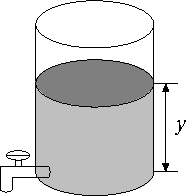
\includegraphics[scale=1]{figure/fig1-8-1.pdf}
			\caption{}\label{fig:1.8.1}
		\end{figure}
		\begin{enumerate}
			\item 求水面高度 $y$ 对于时间 $t$ 的函数 $y = y(t)$;
			\item 设 $k = \frac{1}{10}$. 当 $t = 0$ 时,$y = 9$. 需要多长时间水桶中的水才能流光?($t$ 的单位是 \si{min},$y$ 的单位是 \si{m})
		\end{enumerate}
	\end{ti}

	\begin{ti}
		正方体冰块放在空气中,其边长为 $m$,在温度恒定的情况下,冰块的融化速度(即体积减少速度)与冰块的表面积成正比,比例常数为 $k > 0$. 假设冰块在融化过程中始终保持正方体形状. 经过一个小时的融化,冰块的体积减小了四分之一. 求冰块完全融化需要的时间.
	\end{ti}